%%%%%%%%%%%%%%%%%%%%%%%%%%%%% Define Article %%%%%%%%%%%%%%%%%%%%%%%%%%%%%%%%%%
\documentclass{article}
%%%%%%%%%%%%%%%%%%%%%%%%%%%%%%%%%%%%%%%%%%%%%%%%%%%%%%%%%%%%%%%%%%%%%%%%%%%%%%%

%%%%%%%%%%%%%%%%%%%%%%%%%%%%% Using Packages %%%%%%%%%%%%%%%%%%%%%%%%%%%%%%%%%%
\usepackage[utf8]{inputenc}
\usepackage{float}
\usepackage{geometry}
\usepackage{amssymb}
\usepackage{amsthm}
\usepackage{amsmath}
\usepackage{graphicx}
\usepackage[breaklinks]{hyperref}
\usepackage{listings}
\usepackage{fancyhdr}
\usepackage[english]{babel}
\usepackage{mdframed}
\usepackage{lipsum}
\usepackage{color}
\usepackage{psfrag}
\usepackage{pgfplots}
\usepackage{titlesec}
\usepackage{cite}
\usepackage{hyperref}
\usepackage{tabularx}

%%%%%%%%%%%%%%%%%%%%%%%%%%%%%%%%%%%%%%%%%%%%%%%%%%%%%%%%%%%%%%%%%%%%%%%%%%%%%%%

%%%%%%%%%%%%%%%%%%%%%%%%%% C Code Listing Settings %%%%%%%%%%%%%%%%%%%%%%%%%%%%%%%%%%%%%%%
\definecolor{mGreen}{rgb}{0.25,0.63,0.15}
\definecolor{mGray}{rgb}{0.5,0.5,0.5}
\definecolor{mPurple}{rgb}{0.58,0,0.82}
\definecolor{codeBlue}{rgb}{0.01, 0.2, 0.92}
\definecolor{codegray}{rgb}{0.5,0.5,0.5}
\definecolor{codepurple}{rgb}{0.58,0,0.82}
\definecolor{codeblue}{rgb}{0.13,0.29,0.53}
\definecolor{backgroundColour}{rgb}{0.95,0.95,0.95}

\lstset{
    backgroundcolor=\color{backgroundColour},   
    commentstyle=\color{deepGreen},
    keywordstyle=\color{blue},
    numberstyle=\tiny\color{mGray},
    stringstyle=\color{red},
    basicstyle=\ttfamily\small,
    breakatwhitespace=false,
    breaklines=true,
    captionpos=b,
    keepspaces=true,
    numbers=left,
    numbersep=5pt,
    showspaces=false,
    showstringspaces=false,
    showtabs=false,
    tabsize=2,
    language=C,
    frame=single
}


%%%%%%%%%%%%%%%%%%%%%%%%%%%%%%%%%%%%%%%%%%%%%%%%%%%%%%%%%%%%%%%%%%%%%%%%%%%%%%%

% Other Settings
\hypersetup{
    colorlinks = true,
    linkcolor = black,
    urlcolor = blue,
}
\urlstyle{same}

%%%%%%%%%%%%%%%%%%%%%%%%%% Page Setting %%%%%%%%%%%%%%%%%%%%%%%%%%%%%%%%%%%%%%%
\geometry{a4paper}
\pagestyle{fancy}
\fancyhead{}
\fancyhead[L]{CS232 - Operating Systems}
\fancyhead[C]{Assignment 02 - Report}
\fancyhead[R]{}
\fancyfoot{}
\fancyfoot[C]{\thepage}

%%%%%%%%%%%%%%%%%%%%%%%%%% Define some useful colors %%%%%%%%%%%%%%%%%%%%%%%%%%
\definecolor{ocre}{RGB}{243,102,25}
\definecolor{mygray}{RGB}{243,243,244}
\definecolor{deepGreen}{RGB}{26,111,0}
\definecolor{shallowGreen}{RGB}{235,255,255}
\definecolor{deepBlue}{RGB}{61,124,222}
\definecolor{shallowBlue}{RGB}{235,249,255}
%%%%%%%%%%%%%%%%%%%%%%%%%%%%%%%%%%%%%%%%%%%%%%%%%%%%%%%%%%%%%%%%%%%%%%%%%%%%%%%

%%%%%%%%%%%%%%%%%%%%%%%%%% Define an orangebox command %%%%%%%%%%%%%%%%%%%%%%%%
\newcommand\orangebox[1]{\fcolorbox{ocre}{mygray}{\hspace{1em}#1\hspace{1em}}}
%%%%%%%%%%%%%%%%%%%%%%%%%%%%%%%%%%%%%%%%%%%%%%%%%%%%%%%%%%%%%%%%%%%%%%%%%%%%%%%

%%%%%%%%%%%%%%%%%%%%%%%%%%%% English Environments %%%%%%%%%%%%%%%%%%%%%%%%%%%%%
\newtheoremstyle{mytheoremstyle}{3pt}{3pt}{\normalfont}{0cm}{\rmfamily\bfseries}{}{1em}{{\color{black}\thmname{#1}~\thmnumber{#2}}\thmnote{\,--\,#3}}
\newtheoremstyle{myproblemstyle}{3pt}{3pt}{\normalfont}{0cm}{\rmfamily\bfseries}{}{1em}{{\color{black}\thmname{#1}~\thmnumber{#2}}\thmnote{\,--\,#3}}
\theoremstyle{mytheoremstyle}
\newmdtheoremenv[linewidth=1pt,backgroundcolor=shallowGreen,linecolor=deepGreen,leftmargin=0pt,innerleftmargin=20pt,innerrightmargin=20pt,]{theorem}{Theorem}[section]
\theoremstyle{mytheoremstyle}
\newmdtheoremenv[linewidth=1pt,backgroundcolor=shallowBlue,linecolor=deepBlue,leftmargin=0pt,innerleftmargin=20pt,innerrightmargin=20pt,]{definition}{Definition}[section]
\theoremstyle{myproblemstyle}
\newmdtheoremenv[linecolor=black,leftmargin=0pt,innerleftmargin=10pt,innerrightmargin=10pt,]{problem}{Problem}[section]
%%%%%%%%%%%%%%%%%%%%%%%%%%%%%%%%%%%%%%%%%%%%%%%%%%%%%%%%%%%%%%%%%%%%%%%%%%%%%%%

\title{{\huge \textbf{Habib University \\ Operating Systems - CS232 }}

\vspace*{5mm}
{\LARGE \textbf{Assignment 02 - Report}} \\ 
{\Large \textbf{Simulating A Scheduler}}

% {\Large \textbf{Project Report / Project Title}} \\
{\includegraphics[width=0.75\linewidth]{logo.png}} \\ 
{\Large \textbf{Instructor:} Munzir Zafar}}
\author{Ali Muhammad Asad - aa07190}
\date{}

\pgfplotsset{compat=1.18}

\begin{document}
\maketitle

\newpage
\tableofcontents

\newpage
\section{Introduction}
The assignment is to write a simulator for a process scheduler using C language. Processes will be given to the program on the command line terminal, along with the scheduling algorithm to use, then the program will select the given processing algorithm to manage the processes with. A queue data structure has been made to store the processes based on time of arrival, and this queue will be passed as an argument to the scheduler along with the system time (by default it is always 0 thus a scheduler always starts from 0 system time).

The scheduling algorithms are FIFO (First-In-First-Out), SJF (Shortest Job First), STCF (Shortest Time to Completion First), and RR (Round Robin).

\section{Makefile}
The accompanying makefile has also been provided with the program, and supports the following commands: \vspace*{-1mm}
\begin{itemize}
  \item[-] \texttt{make build}: builds the program and creates an executable file \texttt{scheduler} \vspace*{-2mm}
  \item[-] \texttt{make run}: runs the program, input has to be provided on the command line (input format is discussed in the next section) \vspace*{-2mm}
  \item[-] \texttt{make clean}: removes the executable file \texttt{scheduler}
\end{itemize}

\section{Input}
The input is given in the command line / terminal. The first line will be the total number $N$ of processes \texttt{(int)}, followed by the scheduling policy \texttt{(string)} in the second line which could be one of \textrm{FIFO, SJF, STCF, RR}. Then $N$ lines of input will follow, each containing the following data separated by colon \texttt{(:)}; Process Name \texttt{pname}, Process ID \texttt{pid}, Process total runtime \texttt{duration}, and Process Arrival Time \texttt{arrivaltime}. \texttt{pname} will be a string of upto 10 chars, all other fields will be integers.

\noindent A Sample Input is as follows:

\vspace*{2mm}
\noindent\texttt{3} \\
\texttt{RR} \\
\texttt{P1:12:7:3} \\
\texttt{P2:15:3:5} \\
\texttt{P3:1:6:2} \\
\texttt{end} \vspace*{3mm}

The last line \texttt{end} is just there to show there are no more processes, you can replace it with any other string and the program will still work. But you do need to provide something after you have given the last process else it won't move forward (courtesy of hackerrank and given code that I won't change).

\newpage
\section{Output}
The program simulates the scheduler at every step, showing the state of the system in the following format: \vspace*{-2mm}
\begin{itemize}
  \item[]\hspace*{-3.25mm}\texttt{time: running name: ready queue names comma separated:}
  \item \texttt{time} represents the clock-ticks passed since the system started (assuing a clock-tick lasts 1 millisecond). System starts at 0 ticks, and a clock tick between 0 and 1 ms is considered as 1 tick.
  \item \texttt{running name} represents the name of the process currently running on the CPU, if no process is running then it will be \texttt{idle}.
  \item \texttt{ready queue names} represents the names of the processes in the ready queue, if the ready queue is empty then it will be \texttt{empty}.
\end{itemize}

\noindent Sample Output for the given sample input:

\noindent\texttt{1:idle:empty:} \\
\texttt{2:idle:empty:} \\
\texttt{3:P3:empty:} \\
\texttt{4:P3:P1(7),:} \\
\texttt{5:P1:P3(4),:} \\
\texttt{6:P3:P1(6),P2(3),:} \\
\texttt{7:P1:P2(3),P3(3),:} \\
\texttt{8:P2:P3(3),P1(5),:} \\
\texttt{9:P3:P1(5),P2(2),:} \\
\texttt{10:P1:P2(2),P3(2),:} \\
\texttt{11:P2:P3(2),P1(4),:} \\
\texttt{12:P3:P1(4),P2(1),:} \\
\texttt{13:P1:P2(1),P3(1),:} \\
\texttt{14:P2:P3(1),P1(3),:} \\
\texttt{15:P3:P1(3),:} \\
\texttt{16:P1:empty:} \\
\texttt{17:P1:empty:} \\
\texttt{18:P1:empty:}

\newpage
\section{Scheduling Algorithms}
Before running into the scheduling algorithms, a change was made to the Process Control Block (PCB) struct, in order to efficiently, and effectively calculate the response time. The PCB struct now contains a boolean variable \texttt{isfirsttime} which is set to true by default, and is set to false when the process is run for the first time. This way, the response time is calculated only once, and not every time the process is run. The PCB struct now looks like this:
\begin{lstlisting}[caption={Struct PCB - Process Control Block},label={lst:pcb}]
struct pcb{                   // stores info on a process
  unsigned int pid;           // pid
  char pname[20];             // pname
  unsigned int ptimeleft;     // time left to complete
  unsigned int ptimearrival;  // time of arrival
  bool isfirsttime;           // flag for first run time check -> true
  unsigned int pfirstruntime; // time when process ran for the first time
}; typedef struct pcb pcb;
\end{lstlisting}

\subsection{FIFO - First In First Out}
\begin{lstlisting}[caption={FIFO Scheduling Algorithm},label={lst:fifo}]
void sched_FIFO(dlq *const p_fq, int *p_time){
  // initialize a queue to manage processes that are ready to run
  dlq queue; queue.head = queue.tail = NULL;
  // initialize the first process node from the head of the queue
  dlq_node *process = remove_from_head(p_fq);

  // initialize performance metrics
  int num_processes = 1;
  int rt1 = 0, response_time = 0;
  int turnaround_time = 0;
  int first_exec = process->data->ptimearrival + 1;

  while(1){
    (*p_time)++; // increment the system time
    // if no processes left to run, and both queues empty, break the loop
    if(!(process->data->ptimeleft) && is_empty(&queue) && is_empty(p_fq))
      break;
    
    // if processes are left and a process has arrived, add it to the queue and increment the number of processes
    if(!is_empty(p_fq) && p_fq->head->data->ptimearrival < (*p_time)){
      add_to_tail(&queue, remove_from_head(p_fq));
      num_processes++;
    }

    if(process->data->isfirsttime == true){ // if the process has not run before, set its first runtime to the system time and set isfirsttime to false
      process->data->isfirsttime = false;
      process->data->pfirstruntime = (*p_time);
      rt1 = (*p_time) - process->data->ptimearrival;
      if (rt1 < 0) rt1 = 1;
      response_time += rt1;
    }

    printf("%d:", (*p_time));
    // if the process still has to arrive, print idle, else decrement its time and print its name
    if(process->data->ptimearrival >= (*p_time))
      printf("idle:");
    else{
      process->data->ptimeleft--;
      printf("%s:", process->data->pname);
    }
    // if the queue is empty, print empty, else show contents of the queue
    if(is_empty(&queue)) printf("empty:\n");
    else{
      print_q(&queue);
      printf(":\n");
    }

    // if process has finished, calculate the turnaround time and add it to the total turnaround time, then remove another process from the queue if queue is not empty
    if(process->data->ptimeleft == 0){
      turnaround_time += (*p_time) - process->data->ptimearrival;
      if (!is_empty(&queue))
        process = remove_from_head(&queue);
    }
  } free(process);
  float throughput = (float)num_processes / ((*p_time) - first_exec);
  float avg_turnaround_time = (float)turnaround_time / num_processes;
  float avg_response_time = (float)response_time / num_processes;
  printf("Throughput: %.3f\n", throughput);
  printf("Average turnaround time: %.3f\n", avg_turnaround_time);
  printf("Average response time: %.3f\n", avg_response_time);
  return;
}
\end{lstlisting}
The FIFO scheduling algorithm is the simplest of all, it just runs the processes in the order they arrive. The processes are stored in a queue, and the first process is removed from the head of the queue and run. If the process has not run before, its first runtime is set to the current system time, and the response time is calculated. The process is then run for 1 tick, and if it has finished, the turnaround time is calculated and the next process is removed from the queue. If the process has not finished, it is kept running until it finishes. If the queue is empty, the process is kept running until it finishes. If the queue is not empty, the next process is removed from the queue and run. This process is repeated until all processes have finished running, and both queues become empty. Then the performance metrics are used to calculate the average turnaround time, average response time, and throughput which is then printed out, and the function returns.

\subsection{SJF - Shortest Job First}
\begin{lstlisting}[caption={SJF Scheduling Algorithm},label={lst:sjf}]
void sched_SJF(dlq *const p_fq, int *p_time){
  dlq queue; queue.head = queue.tail = NULL;
  dlq_node *process = remove_from_head(p_fq);

  int num_processes = 1, rt1 = 0, response_time = 0, turnaround_time = 0, first_exec = process->data->ptimearrival + 1;

  while(1){
    (*p_time)++;

    if(!(process->data->ptimeleft) && is_empty(&queue) && is_empty(p_fq))
      break;
    // if processes left with arrival time less than system time, add them to the tail of the queue, and sort by time to completion
    if(!is_empty(p_fq) && p_fq->head->data->ptimearrival < (*p_time)){
      add_to_tail(&queue, remove_from_head(p_fq));
      num_processes++;
      sort_by_timetocompletion(&queue);
    }

    if(process->data->isfirsttime == true){
      process->data->isfirsttime = false;
      process->data->pfirstruntime = (*p_time);
      rt1 = (*p_time) - process->data->ptimearrival;
      if (rt1 < 0) rt1 = 1;
      response_time += rt1;
    }

    printf("%d:", *p_time);
    // if process still has to arrive, print idle, else decrement its time and print its name
    if(process->data->ptimearrival >= (*p_time)) printf("idle:");
    else{
      process->data->ptimeleft--;
      printf("%s:", process->data->pname);
    }
    // if queue is empty, print empty, else show contents of the queue
    if(is_empty(&queue)) printf("empty:\n");
    else{
      print_q(&queue);
      printf(":\n");
    }

    if(process->data->ptimeleft == 0){
      turnaround_time += (*p_time) - process->data->ptimearrival;
      if(!is_empty(&queue))
        process = remove_from_head(&queue);
    }
  }
  free(process);
  float throughput = (float)num_processes / ((*p_time) - first_exec);
  float avg_turnaround_time = (float)turnaround_time / num_processes;
  float avg_response_time = (float)response_time / num_processes;
  printf("Throughput: %.3f\n", throughput);
  printf("Average turnaround time: %.3f\n", avg_turnaround_time);
  printf("Average response time: %.3f\n", avg_response_time);
  return;
}
\end{lstlisting}
The Shortest Job First (SJF) algorithm derives from the FIFO algorithm. When a process arrives and is added to the ready queue, the queue is sorted by time to completion. Therefore, when the current process ends, the next process to run will be the one that has the shortest completion time. This simulates the shortest job first algorithm as the shortest job will always be the next one to run. The rest of the algorithm is the same as FIFO, and the performance metrics are calculated and printed at the end.

\subsection{STCF - Shortest Time to Completion First}
\begin{lstlisting}[caption={STCF Scheduling Algorithm},label={lst:stcf}]
void sched_STCF(dlq *const p_fq, int *p_time){
  dlq queue; queue.head = queue.tail = NULL;
  dlq_node *process = remove_from_head(p_fq);

  int num_processes = 1, rt1 = 0, response_time = 0, turnaround_time = 0, first_exec = process->data->ptimearrival + 1;

  while(1){
    (*p_time)++;
    if(!(process->data->ptimeleft) && is_empty(&queue) && is_empty(p_fq))
      break;

    if(!is_empty(p_fq) && p_fq->head->data->ptimearrival < (*p_time)){
      add_to_tail(&queue, remove_from_head(p_fq));
      num_processes++;
    }

    if(process->data->isfirsttime == true){
      process->data->isfirsttime = false;
      process->data->pfirstruntime = (*p_time);
      rt1 = (*p_time) - process->data->ptimearrival;
      if (rt1 < 0) rt1 = 1;
      response_time += rt1;
    }

    sort_by_timetocompletion(&queue); // sort the queue by time to completion

    printf("%d:", *p_time);
    if(process->data->ptimearrival >= (*p_time))
      printf("idle:");
    else{
      if(!is_empty(&queue) && (process->data->ptimeleft > queue.head->data->ptimeleft)){
        add_to_tail(&queue, process);
        process = remove_from_head(&queue);
      }
      if(process->data->isfirsttime == false){
        process->data->isfirsttime = true;
        process->data->pfirstruntime = (*p_time);
        rt1 = (*p_time) - process->data->ptimearrival;
        if (rt1 < 0) rt1 = 1;
        response_time += rt1;
      }
      process->data->ptimeleft--;
      printf("%s:", process->data->pname);
    }

    if(is_empty(&queue))
      printf("empty:\n");
    else{
      sort_by_timetocompletion(&queue);
      print_q(&queue);
      printf(":\n");
    }

    if(process->data->ptimeleft == 0){
      turnaround_time += (*p_time) - process->data->ptimearrival;
      if(!is_empty(&queue))
        process = remove_from_head(&queue);
    }
  }
  free(process);
  float throughput = (float)num_processes / ((*p_time) - first_exec);
  float avg_turnaround_time = (float)turnaround_time / num_processes;
  float avg_response_time = (float)response_time / num_processes;
  printf("Throughput: %.3f\n", throughput);
  printf("Average turnaround time: %.3f\n", avg_turnaround_time);
  printf("Average response time: %.3f\n", avg_response_time);
  return;
}
\end{lstlisting}
The Shortest Time to Completion First (STCF) is a modification of the SJF algorithm. The ready queue is sorted by time to completion, and the process with the shortest time to completion is run. If a process arrives with a shorter time to completion than the current process, the current process is added to the tail of the queue and the new process is run (the queue is again sorted based on time to completion so that the shortest algorithm is run next). The performance metrics are then calculated and printed at the end.

\pagebreak
\subsection{RR - Round Robin}
\begin{lstlisting}[caption={RR Scheduling Algorithm},label={lst:rr}]
void sched_RR(dlq *const p_fq, int *p_time){
  dlq queue; queue.head = queue.tail = NULL;
  dlq_node *process = remove_from_head(p_fq);
  int quantum_time = 1, process_time = 0; // quantum is the time slice for each process, process_time is the time the process has been running

  int num_processes = 1, rt1 = 0, response_time = 0, turnaround_time = 0, first_exec = process->data->ptimearrival + 1;

  while(1){
    (*p_time)++;
    if (!(process->data->ptimeleft) && is_empty(&queue) && is_empty(p_fq))
      break;

    if(!is_empty(p_fq) && p_fq->head->data->ptimearrival < (*p_time)){
      add_to_tail(&queue, remove_from_head(p_fq));
      num_processes++;
    }

    if(process->data->isfirsttime == true){
      process->data->isfirsttime = false;
      process->data->pfirstruntime = (*p_time);
      rt1 = (*p_time) - process->data->ptimearrival;
      if (rt1 < 0) rt1 = 1;
      response_time += rt1;
    }

    printf("%d:", *p_time);
    if(process->data->ptimearrival >= (*p_time))
      printf("idle:");
    else{ // if process has arrived, decrement its time, update the time it has run for, and print its name
      process->data->ptimeleft--;
      process_time++;
      printf("%s:", process->data->pname);
    }

    if(is_empty(&queue))
      printf("empty:\n");
    else{
      print_q(&queue);
      printf(":\n");
    }

    if(process->data->ptimeleft == 0){
      turnaround_time += (*p_time) - process->data->ptimearrival;
      if (!is_empty(&queue))
        process = remove_from_head(&queue);
    }

    if(process_time == quantum_time){ // if process has run for the time slice, add it to the tail of the queue and set process_time to 0
      add_to_tail(&queue, process);
      process = remove_from_head(&queue);
      process_time = 0;
    }
  }
  free(process);
  float throughput = (float)num_processes / ((*p_time) - first_exec);
  float avg_turnaround_time = (float)turnaround_time / num_processes;
  float avg_response_time = (float)response_time / num_processes;
  printf("Throughput: %.3f\n", throughput);
  printf("Average turnaround time: %.3f\n", avg_turnaround_time);
  printf("Average response time: %.3f\n", avg_response_time);
  return;
}    
\end{lstlisting}
The Round Robin (RR) is a modification of the FIFO code. A quantum time slice is set to 1 tick, and each process is run for the  time slice. (The quantim time slice can be changed as per preference). On each iteration, the process time is set to 0, and incremented once a process has run. If the process has run for the time slice, it is added to the tail of the queue and the next process is run. If the process has completed, it is removed from the queue and the next process is run (process time is set to 0). The performance metrics are then calculated and printed at the end.

\newpage
\section{Performance Metrics of Scheduling Algorithms}
% Over Here goes some details on performance metrics blah blah blah
Each of the four scheduling algorithms are run over some sample test cases, and the performance metrics are calculated for each of them. More specifically, the metrics being measured are: \vspace*{-2mm}
\begin{enumerate}
  \item Average Throughput of the scheduler \vspace*{-2mm}
  \item Average Response Time of the scheduler \vspace*{-2mm}
  \item Average Turnaround Time of the scheduler
\end{enumerate}

Outputs have been attached in the appendix for each of the test cases, and the performance metrics have been calculated and tabulated in the following sections.

\vspace*{2mm}
\noindent \textit{*For each test case, green highlight indicates best performance, and red highlight indicates worst performance.}

\subsection{Testing Performance Metrics}
\subsubsection{Test Case 0 / Test Case 2 (same test case)}
Sample Input: \vspace*{2mm}

\noindent\texttt{3} \\
\texttt{\textit{Scheduling Algorithm}} \\
\texttt{P1:12:7:3} \\
\texttt{P2:15:3:5} \\
\texttt{P3:1:6:2}

\begin{figure}[htbp]
  \centering
  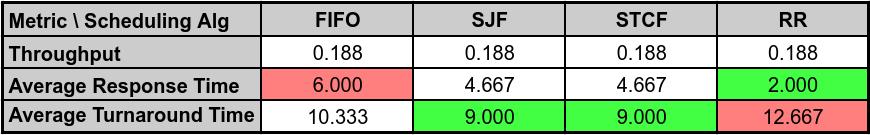
\includegraphics[width=\textwidth]{tc1.png}

  \vspace*{2mm}
  Table 1: Test Case 0 / Test Case 2 Performance Metrics
\end{figure}

The above table shows that the throughput remains the same throuhgout which is logical as the number of processes and the time taken by each process, in essence, remains same. In terms of average response time, RR performs better for this test case, while SJF and STCF have the same average turnaround time for this test case.
\pagebreak
\subsubsection{Test Case 5}
Sample Input: \vspace*{2mm}

\noindent\texttt{6} \\
\texttt{\textit{Scheduling Algorithm}} \\
\texttt{P1:1:5:0} \\
\texttt{P2:2:7:2} \\
\texttt{P3:3:6:3} \\
\texttt{P4:4:9:4} \\
\texttt{P5:5:8:5} \\
\texttt{P6:6:4:7}

\begin{figure}[htbp]
  \centering
  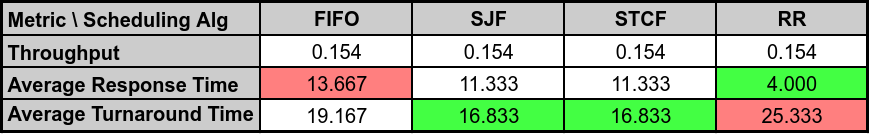
\includegraphics[width=\textwidth]{tc2.png}

  \vspace*{2mm}
  Table 2: Test Case 5 Performance Metrics
\end{figure}

Again, the throughput remains same throughout, average response time is best for RR, and average turnaround time is best for SJF and STCF.

\subsubsection{Test Case 10}
Sample Input: \vspace*{2mm}

\noindent\texttt{6} \\
\texttt{\textit{Scheduling Algorithm}} \\
\texttt{P1:1:6:0} \\
\texttt{P2:2:12:2} \\
\texttt{P3:3:8:4} \\
\texttt{P4:4:15:5} \\
\texttt{P5:5:5:7} \\
\texttt{P6:6:10:9}

\begin{figure}[htbp]
  \centering
  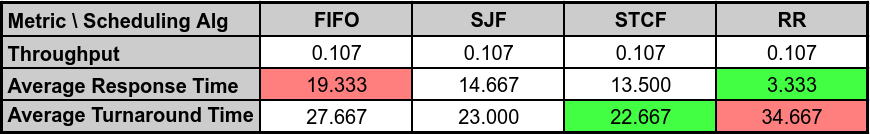
\includegraphics[width=\textwidth]{tc3.png}

  \vspace*{2mm}
  Table 3: Test Case 10 Performance Metrics
\end{figure}

Again, the throughput remains same throughout, average response time is best for RR, and average turnaround time is almost the same for SJF and STCF, however, STCF performs slightly better. Hence, STCF has the best average response time for this test case8.

\subsubsection{Test Case 13}
Sample Input: \vspace*{2mm}

\noindent\texttt{8} \\
\texttt{\textit{Scheduling Algorithm}} \\
\texttt{P1:1:10:0} \\
\texttt{P2:2:15:2} \\
\texttt{P3:3:8:4} \\
\texttt{P4:4:12:6} \\
\texttt{P5:5:6:9} \\
\texttt{P6:6:4:11} \\
\texttt{P7:7:7:13} \\
\texttt{P8:8:9:15}

\begin{figure}[htbp]
  \centering
  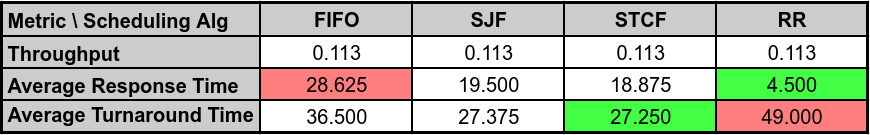
\includegraphics[width=\textwidth]{tc4.png}

  \vspace*{2mm}
  Table 4: Test Case 13 Performance Metrics
\end{figure}

\vspace*{-2mm}
Again, the throughput remains same throughout, average response time is best for RR, and average turnaround time is best for STCF.


\subsection{Results - Comparison of Performance Metrics}

% From the above results, we can conlude the following:
% \begin{itemize}
%   \item The throughput remains the same for all scheduling algorithms for any particular test case, which is quite logical since the number of processes and the time taken by each process remains the same. Hence, the cumulative sum for the execution time should remain same.
%   \item The average response time is best for RR in all test cases, which is also logical since RR ensures that each process gets a fair share of the CPU time as it executes in a round robin manner, hence the response time is best for RR.
%   \item The average turnaround time is best for STCF in all test cases (slightly performing better than SJF in some while having the same turnaround as SJF in others - but not less than SJF). This is also logical since STCF ensures that the process with the shortest time to completion is run first, regardless of the order of arrival, and if any other process is running; if a new process can be finished first, then it is executed. Therefore, the average completion time is best for STCF.
% \end{itemize}

From the above results, a cumulative results table can be made:
\begin{figure}[htbp]
  \centering
  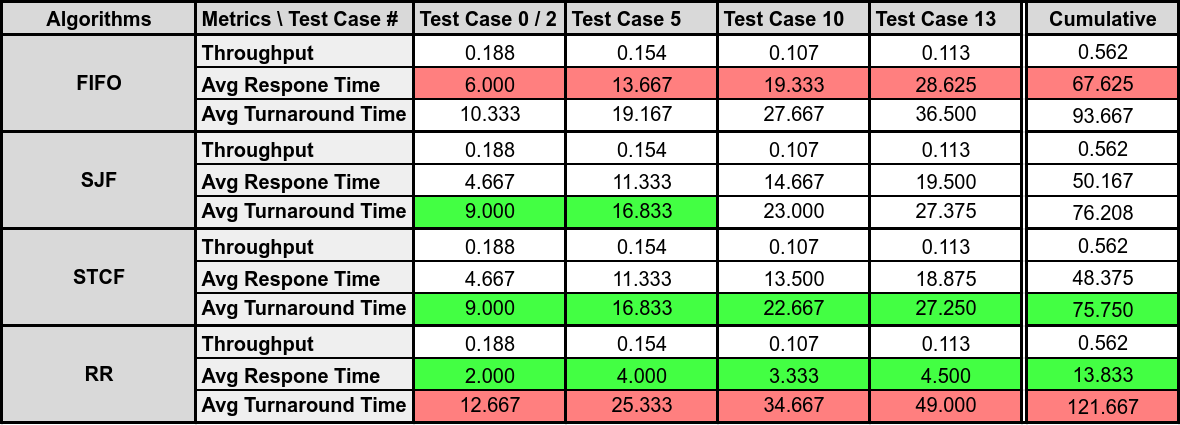
\includegraphics[width=\textwidth]{overall.png}

  \vspace*{2mm}
  Table 5: Cumulative Overall Performance Metrics
\end{figure} \vspace*{-2mm}

\begin{itemize}
  \item \textbf{Best Throughput:} Remains same for all which is logical since cumulatively, all processes in a test case will have the same total time regardless of the algorithm used. \vspace*{-2mm}
  \item \textbf{Best Avg Response Time:} \textit{Round Robin}, which is logical since RR ensures that each process gets a fair share of the CPU time as it executes in a round robin manner. \vspace*{-2mm}
  \item \textbf{Best Avg Turnaround Time:} \textit{STCF}; again logical since STCF ensures a process with lesser runtime runs first even if a process is currently running.
\end{itemize}

% \noindent \textbf{Best Average Throughput?} \textit{Same for all schedules} \vspace*{2mm}

% \noindent \textbf{Best Average Response Time?} \textit{RR} \vspace*{2mm}

% \noindent \textbf{Best Average Turnaround Time?} \textit{STCF}

\newpage
\section{Takeaway and Reflections}

This homework was significantly, comparatively, much easier. It was a great learning experience about implementing the different scheduling algorithms and then modifying them to compute their performance metrics to find out which algorithms performs better with regards to which aspect. It was fun and interesting.

\begin{figure}[htbp]
  \centering
  
\includegraphics[width=0.35\textwidth]{kawaiii.jpeg}
\end{figure}

\newpage
\section{References}
\begin{thebibliography}{9}
  \bibitem{coursebook}
  Remzi H. Arpaci-Desseau and Andrea C. Arpaci-Desseau.
  \textit{Operating Systems: Three Easy Pieces}.
  Arpaci-Dusseau Books, LLC, 2015.

  \bibitem{ChatGPT}
  \textit{ChatGPT}. [Online]. Available: \url{https://chat.openai.com/} mainly for understanding, resolving errors, and commentation.

  \bibitem{Bing AI}
  \textit{Bing AI ChatBot}. [Online]. Available: \url{https://www.bing.com/search?toWww=1&redig=0011FC72B09C43A9A833284287211CB9&q=Bing+AI&showconv=1} mainly for understanding, resolving errors, and commentation. (Open with Microsoft Edge)
\end{thebibliography}

\newpage
\appendix
\section{Appendix}

\subsection{Outputs for Test Cases}
\subsubsection{Test Case 0 / Test Case 2}
\noindent \textbf{FIFO}
\begin{verbatim}
1:idle:empty:
2:idle:empty:
3:P3:empty:
4:P3:P1(7),:
5:P3:P1(7),:
6:P3:P1(7),P2(3),:
7:P3:P1(7),P2(3),:
8:P3:P1(7),P2(3),:
9:P1:P2(3),:
10:P1:P2(3),:
11:P1:P2(3),:
12:P1:P2(3),:
13:P1:P2(3),:
14:P1:P2(3),:
15:P1:P2(3),:
16:P2:empty:
17:P2:empty:
18:P2:empty:
Throughput: 0.188
Average turnaround time: 10.333
Average response time: 6.000
\end{verbatim}

\noindent \textbf{SJF}
\begin{verbatim}
1:idle:empty:
2:idle:empty:
3:P3:empty:
4:P3:P1(7),:
5:P3:P1(7),:
6:P3:P2(3),P1(7),:
7:P3:P2(3),P1(7),:
8:P3:P2(3),P1(7),:
9:P2:P1(7),:
10:P2:P1(7),:
11:P2:P1(7),:
12:P1:empty:
13:P1:empty:
14:P1:empty:
15:P1:empty:
16:P1:empty:
17:P1:empty:
18:P1:empty:
Throughput: 0.188
Average turnaround time: 9.000
Average response time: 4.667
\end{verbatim}

\noindent \textbf{STCF}
\begin{verbatim}
1:idle:empty:
2:idle:empty:
3:P3:empty:
4:P3:P1(7),:
5:P3:P1(7),:
6:P3:P2(3),P1(7),:
7:P3:P2(3),P1(7),:
8:P3:P2(3),P1(7),:
9:P2:P1(7),:
10:P2:P1(7),:
11:P2:P1(7),:
12:P1:empty:
13:P1:empty:
14:P1:empty:
15:P1:empty:
16:P1:empty:
17:P1:empty:
18:P1:empty:
Throughput: 0.188
Average turnaround time: 9.000
Average response time: 4.667
\end{verbatim}

\noindent \textbf{RR}
\begin{verbatim}
1:idle:empty:
2:idle:empty:
3:P3:empty:
4:P3:P1(7),:
5:P1:P3(4),:
6:P3:P1(6),P2(3),:
7:P1:P2(3),P3(3),:
8:P2:P3(3),P1(5),:
9:P3:P1(5),P2(2),:
10:P1:P2(2),P3(2),:
11:P2:P3(2),P1(4),:
12:P3:P1(4),P2(1),:
13:P1:P2(1),P3(1),:
14:P2:P3(1),P1(3),:
15:P1:P3(1),:
16:P3:P1(2),:
17:P1:empty:
18:P1:empty:
Throughput: 0.188
Average turnaround time: 12.667
Average response time: 2.000
\end{verbatim}

\subsubsection{Test Case 5}
\noindent \textbf{FIFO}
\begin{verbatim}
1:P1:empty:
2:P1:empty:
3:P1:P2(7),:
4:P1:P2(7),P3(6),:
5:P1:P2(7),P3(6),P4(9),:
6:P2:P3(6),P4(9),P5(8),:
7:P2:P3(6),P4(9),P5(8),:
8:P2:P3(6),P4(9),P5(8),P6(4),:
9:P2:P3(6),P4(9),P5(8),P6(4),:
10:P2:P3(6),P4(9),P5(8),P6(4),:
11:P2:P3(6),P4(9),P5(8),P6(4),:
12:P2:P3(6),P4(9),P5(8),P6(4),:
13:P3:P4(9),P5(8),P6(4),:
14:P3:P4(9),P5(8),P6(4),:
15:P3:P4(9),P5(8),P6(4),:
16:P3:P4(9),P5(8),P6(4),:
17:P3:P4(9),P5(8),P6(4),:
18:P3:P4(9),P5(8),P6(4),:
19:P4:P5(8),P6(4),:
20:P4:P5(8),P6(4),:
21:P4:P5(8),P6(4),:
22:P4:P5(8),P6(4),:
23:P4:P5(8),P6(4),:
24:P4:P5(8),P6(4),:
25:P4:P5(8),P6(4),:
26:P4:P5(8),P6(4),:
27:P4:P5(8),P6(4),:
28:P5:P6(4),:
29:P5:P6(4),:
30:P5:P6(4),:
31:P5:P6(4),:
32:P5:P6(4),:
33:P5:P6(4),:
34:P5:P6(4),:
35:P5:P6(4),:
36:P6:empty:
37:P6:empty:
38:P6:empty:
39:P6:empty:
Throughput: 0.154
Average turnaround time: 19.167
Average response time: 13.667
\end{verbatim}

\noindent \textbf{SJF}
\begin{verbatim}
1:P1:empty:
2:P1:empty:
3:P1:P2(7),:
4:P1:P3(6),P2(7),:
5:P1:P3(6),P2(7),P4(9),:
6:P3:P2(7),P5(8),P4(9),:
7:P3:P2(7),P5(8),P4(9),:
8:P3:P6(4),P2(7),P5(8),P4(9),:
9:P3:P6(4),P2(7),P5(8),P4(9),:
10:P3:P6(4),P2(7),P5(8),P4(9),:
11:P3:P6(4),P2(7),P5(8),P4(9),:
12:P6:P2(7),P5(8),P4(9),:
13:P6:P2(7),P5(8),P4(9),:
14:P6:P2(7),P5(8),P4(9),:
15:P6:P2(7),P5(8),P4(9),:
16:P2:P5(8),P4(9),:
17:P2:P5(8),P4(9),:
18:P2:P5(8),P4(9),:
19:P2:P5(8),P4(9),:
20:P2:P5(8),P4(9),:
21:P2:P5(8),P4(9),:
22:P2:P5(8),P4(9),:
23:P5:P4(9),:
24:P5:P4(9),:
25:P5:P4(9),:
26:P5:P4(9),:
27:P5:P4(9),:
28:P5:P4(9),:
29:P5:P4(9),:
30:P5:P4(9),:
31:P4:empty:
32:P4:empty:
33:P4:empty:
34:P4:empty:
35:P4:empty:
36:P4:empty:
37:P4:empty:
38:P4:empty:
39:P4:empty:
Throughput: 0.154
Average turnaround time: 16.833
Average response time: 11.333
\end{verbatim}

\noindent \textbf{STCF}
\begin{verbatim}
1:P1:empty:
2:P1:empty:
3:P1:P2(7),:
4:P1:P3(6),P2(7),:
5:P1:P3(6),P2(7),P4(9),:
6:P3:P2(7),P5(8),P4(9),:
7:P3:P2(7),P5(8),P4(9),:
8:P3:P6(4),P2(7),P5(8),P4(9),:
9:P3:P6(4),P2(7),P5(8),P4(9),:
10:P3:P6(4),P2(7),P5(8),P4(9),:
11:P3:P6(4),P2(7),P5(8),P4(9),:
12:P6:P2(7),P5(8),P4(9),:
13:P6:P2(7),P5(8),P4(9),:
14:P6:P2(7),P5(8),P4(9),:
15:P6:P2(7),P5(8),P4(9),:
16:P2:P5(8),P4(9),:
17:P2:P5(8),P4(9),:
18:P2:P5(8),P4(9),:
19:P2:P5(8),P4(9),:
20:P2:P5(8),P4(9),:
21:P2:P5(8),P4(9),:
22:P2:P5(8),P4(9),:
23:P5:P4(9),:
24:P5:P4(9),:
25:P5:P4(9),:
26:P5:P4(9),:
27:P5:P4(9),:
28:P5:P4(9),:
29:P5:P4(9),:
30:P5:P4(9),:
31:P4:empty:
32:P4:empty:
33:P4:empty:
34:P4:empty:
35:P4:empty:
36:P4:empty:
37:P4:empty:
38:P4:empty:
39:P4:empty:
Throughput: 0.154
Average turnaround time: 16.833
Average response time: 11.333
\end{verbatim}

\noindent \textbf{RR}
\begin{verbatim}
1:P1:empty:
2:P1:empty:
3:P1:P2(7),:
4:P2:P1(2),P3(6),:
5:P1:P3(6),P2(6),P4(9),:
6:P3:P2(6),P4(9),P1(1),P5(8),:
7:P2:P4(9),P1(1),P5(8),P3(5),:
8:P4:P1(1),P5(8),P3(5),P2(5),P6(4),:
9:P1:P5(8),P3(5),P2(5),P6(4),P4(8),:
10:P3:P2(5),P6(4),P4(8),P5(8),:
11:P2:P6(4),P4(8),P5(8),P3(4),:
12:P6:P4(8),P5(8),P3(4),P2(4),:
13:P4:P5(8),P3(4),P2(4),P6(3),:
14:P5:P3(4),P2(4),P6(3),P4(7),:
15:P3:P2(4),P6(3),P4(7),P5(7),:
16:P2:P6(3),P4(7),P5(7),P3(3),:
17:P6:P4(7),P5(7),P3(3),P2(3),:
18:P4:P5(7),P3(3),P2(3),P6(2),:
19:P5:P3(3),P2(3),P6(2),P4(6),:
20:P3:P2(3),P6(2),P4(6),P5(6),:
21:P2:P6(2),P4(6),P5(6),P3(2),:
22:P6:P4(6),P5(6),P3(2),P2(2),:
23:P4:P5(6),P3(2),P2(2),P6(1),:
24:P5:P3(2),P2(2),P6(1),P4(5),:
25:P3:P2(2),P6(1),P4(5),P5(5),:
26:P2:P6(1),P4(5),P5(5),P3(1),:
27:P6:P4(5),P5(5),P3(1),P2(1),:
28:P5:P3(1),P2(1),P4(5),:
29:P3:P2(1),P4(5),P5(4),:
30:P4:P5(4),P2(1),:
31:P5:P2(1),P4(4),:
32:P2:P4(4),P5(3),:
33:P5:P4(4),:
34:P4:P5(2),:
35:P5:P4(3),:
36:P4:P5(1),:
37:P5:P4(2),:
38:P4:empty:
39:P4:empty:
Throughput: 0.154
Average turnaround time: 25.333
Average response time: 4.000
\end{verbatim}

\subsubsection{Test Case 10}
\noindent \textbf{FIFO}
\begin{verbatim}
1:P1:empty:
2:P1:empty:
3:P1:P2(12),:
4:P1:P2(12),:
5:P1:P2(12),P3(8),:
6:P1:P2(12),P3(8),P4(15),:
7:P2:P3(8),P4(15),:
8:P2:P3(8),P4(15),P5(5),:
9:P2:P3(8),P4(15),P5(5),:
10:P2:P3(8),P4(15),P5(5),P6(10),:
11:P2:P3(8),P4(15),P5(5),P6(10),:
12:P2:P3(8),P4(15),P5(5),P6(10),:
13:P2:P3(8),P4(15),P5(5),P6(10),:
14:P2:P3(8),P4(15),P5(5),P6(10),:
15:P2:P3(8),P4(15),P5(5),P6(10),:
16:P2:P3(8),P4(15),P5(5),P6(10),:
17:P2:P3(8),P4(15),P5(5),P6(10),:
18:P2:P3(8),P4(15),P5(5),P6(10),:
19:P3:P4(15),P5(5),P6(10),:
20:P3:P4(15),P5(5),P6(10),:
21:P3:P4(15),P5(5),P6(10),:
22:P3:P4(15),P5(5),P6(10),:
23:P3:P4(15),P5(5),P6(10),:
24:P3:P4(15),P5(5),P6(10),:
25:P3:P4(15),P5(5),P6(10),:
26:P3:P4(15),P5(5),P6(10),:
27:P4:P5(5),P6(10),:
28:P4:P5(5),P6(10),:
29:P4:P5(5),P6(10),:
30:P4:P5(5),P6(10),:
31:P4:P5(5),P6(10),:
32:P4:P5(5),P6(10),:
33:P4:P5(5),P6(10),:
34:P4:P5(5),P6(10),:
35:P4:P5(5),P6(10),:
36:P4:P5(5),P6(10),:
37:P4:P5(5),P6(10),:
38:P4:P5(5),P6(10),:
39:P4:P5(5),P6(10),:
40:P4:P5(5),P6(10),:
41:P4:P5(5),P6(10),:
42:P5:P6(10),:
43:P5:P6(10),:
44:P5:P6(10),:
45:P5:P6(10),:
46:P5:P6(10),:
47:P6:empty:
48:P6:empty:
49:P6:empty:
50:P6:empty:
51:P6:empty:
52:P6:empty:
53:P6:empty:
54:P6:empty:
55:P6:empty:
56:P6:empty:
Throughput: 0.107
Average turnaround time: 27.667
Average response time: 19.333
\end{verbatim}

\noindent \textbf{SJF}
\begin{verbatim}
1:P1:empty:
2:P1:empty:
3:P1:P2(12),:
4:P1:P2(12),:
5:P1:P3(8),P2(12),:
6:P1:P3(8),P2(12),P4(15),:
7:P3:P2(12),P4(15),:
8:P3:P5(5),P2(12),P4(15),:
9:P3:P5(5),P2(12),P4(15),:
10:P3:P5(5),P6(10),P2(12),P4(15),:
11:P3:P5(5),P6(10),P2(12),P4(15),:
12:P3:P5(5),P6(10),P2(12),P4(15),:
13:P3:P5(5),P6(10),P2(12),P4(15),:
14:P3:P5(5),P6(10),P2(12),P4(15),:
15:P5:P6(10),P2(12),P4(15),:
16:P5:P6(10),P2(12),P4(15),:
17:P5:P6(10),P2(12),P4(15),:
18:P5:P6(10),P2(12),P4(15),:
19:P5:P6(10),P2(12),P4(15),:
20:P6:P2(12),P4(15),:
21:P6:P2(12),P4(15),:
22:P6:P2(12),P4(15),:
23:P6:P2(12),P4(15),:
24:P6:P2(12),P4(15),:
25:P6:P2(12),P4(15),:
26:P6:P2(12),P4(15),:
27:P6:P2(12),P4(15),:
28:P6:P2(12),P4(15),:
29:P6:P2(12),P4(15),:
30:P2:P4(15),:
31:P2:P4(15),:
32:P2:P4(15),:
33:P2:P4(15),:
34:P2:P4(15),:
35:P2:P4(15),:
36:P2:P4(15),:
37:P2:P4(15),:
38:P2:P4(15),:
39:P2:P4(15),:
40:P2:P4(15),:
41:P2:P4(15),:
42:P4:empty:
43:P4:empty:
44:P4:empty:
45:P4:empty:
46:P4:empty:
47:P4:empty:
48:P4:empty:
49:P4:empty:
50:P4:empty:
51:P4:empty:
52:P4:empty:
53:P4:empty:
54:P4:empty:
55:P4:empty:
56:P4:empty:
Throughput: 0.107
Average turnaround time: 23.000
Average response time: 14.667
\end{verbatim}

\noindent \textbf{STCF}
\begin{verbatim}
1:P1:empty:
2:P1:empty:
3:P1:P2(12),:
4:P1:P2(12),:
5:P1:P3(8),P2(12),:
6:P1:P3(8),P2(12),P4(15),:
7:P3:P2(12),P4(15),:
8:P5:P3(7),P2(12),P4(15),:
9:P5:P3(7),P2(12),P4(15),:
10:P5:P3(7),P6(10),P2(12),P4(15),:
11:P5:P3(7),P6(10),P2(12),P4(15),:
12:P5:P3(7),P6(10),P2(12),P4(15),:
13:P3:P6(10),P2(12),P4(15),:
14:P3:P6(10),P2(12),P4(15),:
15:P3:P6(10),P2(12),P4(15),:
16:P3:P6(10),P2(12),P4(15),:
17:P3:P6(10),P2(12),P4(15),:
18:P3:P6(10),P2(12),P4(15),:
19:P3:P6(10),P2(12),P4(15),:
20:P6:P2(12),P4(15),:
21:P6:P2(12),P4(15),:
22:P6:P2(12),P4(15),:
23:P6:P2(12),P4(15),:
24:P6:P2(12),P4(15),:
25:P6:P2(12),P4(15),:
26:P6:P2(12),P4(15),:
27:P6:P2(12),P4(15),:
28:P6:P2(12),P4(15),:
29:P6:P2(12),P4(15),:
30:P2:P4(15),:
31:P2:P4(15),:
32:P2:P4(15),:
33:P2:P4(15),:
34:P2:P4(15),:
35:P2:P4(15),:
36:P2:P4(15),:
37:P2:P4(15),:
38:P2:P4(15),:
39:P2:P4(15),:
40:P2:P4(15),:
41:P2:P4(15),:
42:P4:empty:
43:P4:empty:
44:P4:empty:
45:P4:empty:
46:P4:empty:
47:P4:empty:
48:P4:empty:
49:P4:empty:
50:P4:empty:
51:P4:empty:
52:P4:empty:
53:P4:empty:
54:P4:empty:
55:P4:empty:
56:P4:empty:
Throughput: 0.107
Average turnaround time: 22.667
Average response time: 13.500
\end{verbatim}

\noindent \textbf{RR}
\begin{verbatim}
1:P1:empty:
2:P1:empty:
3:P1:P2(12),:
4:P2:P1(3),:
5:P1:P2(11),P3(8),:
6:P2:P3(8),P1(2),P4(15),:
7:P3:P1(2),P4(15),P2(10),:
8:P1:P4(15),P2(10),P3(7),P5(5),:
9:P4:P2(10),P3(7),P5(5),P1(1),:
10:P2:P3(7),P5(5),P1(1),P4(14),P6(10),:
11:P3:P5(5),P1(1),P4(14),P6(10),P2(9),:
12:P5:P1(1),P4(14),P6(10),P2(9),P3(6),:
13:P1:P4(14),P6(10),P2(9),P3(6),P5(4),:
14:P6:P2(9),P3(6),P5(4),P4(14),:
15:P2:P3(6),P5(4),P4(14),P6(9),:
16:P3:P5(4),P4(14),P6(9),P2(8),:
17:P5:P4(14),P6(9),P2(8),P3(5),:
18:P4:P6(9),P2(8),P3(5),P5(3),:
19:P6:P2(8),P3(5),P5(3),P4(13),:
20:P2:P3(5),P5(3),P4(13),P6(8),:
21:P3:P5(3),P4(13),P6(8),P2(7),:
22:P5:P4(13),P6(8),P2(7),P3(4),:
23:P4:P6(8),P2(7),P3(4),P5(2),:
24:P6:P2(7),P3(4),P5(2),P4(12),:
25:P2:P3(4),P5(2),P4(12),P6(7),:
26:P3:P5(2),P4(12),P6(7),P2(6),:
27:P5:P4(12),P6(7),P2(6),P3(3),:
28:P4:P6(7),P2(6),P3(3),P5(1),:
29:P6:P2(6),P3(3),P5(1),P4(11),:
30:P2:P3(3),P5(1),P4(11),P6(6),:
31:P3:P5(1),P4(11),P6(6),P2(5),:
32:P5:P4(11),P6(6),P2(5),P3(2),:
33:P6:P2(5),P3(2),P4(11),:
34:P2:P3(2),P4(11),P6(5),:
35:P3:P4(11),P6(5),P2(4),:
36:P4:P6(5),P2(4),P3(1),:
37:P6:P2(4),P3(1),P4(10),:
38:P2:P3(1),P4(10),P6(4),:
39:P3:P4(10),P6(4),P2(3),:
40:P6:P2(3),P4(10),:
41:P2:P4(10),P6(3),:
42:P4:P6(3),P2(2),:
43:P6:P2(2),P4(9),:
44:P2:P4(9),P6(2),:
45:P4:P6(2),P2(1),:
46:P6:P2(1),P4(8),:
47:P2:P4(8),P6(1),:
48:P6:P4(8),:
49:P4:empty:
50:P4:empty:
51:P4:empty:
52:P4:empty:
53:P4:empty:
54:P4:empty:
55:P4:empty:
56:P4:empty:
Throughput: 0.107
Average turnaround time: 34.667
Average response time: 3.333
\end{verbatim}

\subsubsection{Test Case 13}
\noindent \textbf{FIFO}
\begin{verbatim}
1:P1:empty:
2:P1:empty:
3:P1:P2(15),:
4:P1:P2(15),:
5:P1:P2(15),P3(8),:
6:P1:P2(15),P3(8),:
7:P1:P2(15),P3(8),P4(12),:
8:P1:P2(15),P3(8),P4(12),:
9:P1:P2(15),P3(8),P4(12),:
10:P1:P2(15),P3(8),P4(12),P5(6),:
11:P2:P3(8),P4(12),P5(6),:
12:P2:P3(8),P4(12),P5(6),P6(4),:
13:P2:P3(8),P4(12),P5(6),P6(4),:
14:P2:P3(8),P4(12),P5(6),P6(4),P7(7),:
15:P2:P3(8),P4(12),P5(6),P6(4),P7(7),:
16:P2:P3(8),P4(12),P5(6),P6(4),P7(7),P8(9),:
17:P2:P3(8),P4(12),P5(6),P6(4),P7(7),P8(9),:
18:P2:P3(8),P4(12),P5(6),P6(4),P7(7),P8(9),:
19:P2:P3(8),P4(12),P5(6),P6(4),P7(7),P8(9),:
20:P2:P3(8),P4(12),P5(6),P6(4),P7(7),P8(9),:
21:P2:P3(8),P4(12),P5(6),P6(4),P7(7),P8(9),:
22:P2:P3(8),P4(12),P5(6),P6(4),P7(7),P8(9),:
23:P2:P3(8),P4(12),P5(6),P6(4),P7(7),P8(9),:
24:P2:P3(8),P4(12),P5(6),P6(4),P7(7),P8(9),:
25:P2:P3(8),P4(12),P5(6),P6(4),P7(7),P8(9),:
26:P3:P4(12),P5(6),P6(4),P7(7),P8(9),:
27:P3:P4(12),P5(6),P6(4),P7(7),P8(9),:
28:P3:P4(12),P5(6),P6(4),P7(7),P8(9),:
29:P3:P4(12),P5(6),P6(4),P7(7),P8(9),:
30:P3:P4(12),P5(6),P6(4),P7(7),P8(9),:
31:P3:P4(12),P5(6),P6(4),P7(7),P8(9),:
32:P3:P4(12),P5(6),P6(4),P7(7),P8(9),:
33:P3:P4(12),P5(6),P6(4),P7(7),P8(9),:
34:P4:P5(6),P6(4),P7(7),P8(9),:
35:P4:P5(6),P6(4),P7(7),P8(9),:
36:P4:P5(6),P6(4),P7(7),P8(9),:
37:P4:P5(6),P6(4),P7(7),P8(9),:
38:P4:P5(6),P6(4),P7(7),P8(9),:
39:P4:P5(6),P6(4),P7(7),P8(9),:
40:P4:P5(6),P6(4),P7(7),P8(9),:
41:P4:P5(6),P6(4),P7(7),P8(9),:
42:P4:P5(6),P6(4),P7(7),P8(9),:
43:P4:P5(6),P6(4),P7(7),P8(9),:
44:P4:P5(6),P6(4),P7(7),P8(9),:
45:P4:P5(6),P6(4),P7(7),P8(9),:
46:P5:P6(4),P7(7),P8(9),:
47:P5:P6(4),P7(7),P8(9),:
48:P5:P6(4),P7(7),P8(9),:
49:P5:P6(4),P7(7),P8(9),:
50:P5:P6(4),P7(7),P8(9),:
51:P5:P6(4),P7(7),P8(9),:
52:P6:P7(7),P8(9),:
53:P6:P7(7),P8(9),:
54:P6:P7(7),P8(9),:
55:P6:P7(7),P8(9),:
56:P7:P8(9),:
57:P7:P8(9),:
58:P7:P8(9),:
59:P7:P8(9),:
60:P7:P8(9),:
61:P7:P8(9),:
62:P7:P8(9),:
63:P8:empty:
64:P8:empty:
65:P8:empty:
66:P8:empty:
67:P8:empty:
68:P8:empty:
69:P8:empty:
70:P8:empty:
71:P8:empty:
Throughput: 0.113
Average turnaround time: 36.500
Average response time: 28.625
\end{verbatim}

\noindent \textbf{SJF}
\begin{verbatim}
1:P1:empty:
2:P1:empty:
3:P1:P2(15),:
4:P1:P2(15),:
5:P1:P3(8),P2(15),:
6:P1:P3(8),P2(15),:
7:P1:P3(8),P4(12),P2(15),:
8:P1:P3(8),P4(12),P2(15),:
9:P1:P3(8),P4(12),P2(15),:
10:P1:P5(6),P3(8),P4(12),P2(15),:
11:P5:P3(8),P4(12),P2(15),:
12:P5:P6(4),P3(8),P4(12),P2(15),:
13:P5:P6(4),P3(8),P4(12),P2(15),:
14:P5:P6(4),P7(7),P3(8),P4(12),P2(15),:
15:P5:P6(4),P7(7),P3(8),P4(12),P2(15),:
16:P5:P6(4),P7(7),P3(8),P8(9),P4(12),P2(15),:
17:P6:P7(7),P3(8),P8(9),P4(12),P2(15),:
18:P6:P7(7),P3(8),P8(9),P4(12),P2(15),:
19:P6:P7(7),P3(8),P8(9),P4(12),P2(15),:
20:P6:P7(7),P3(8),P8(9),P4(12),P2(15),:
21:P7:P3(8),P8(9),P4(12),P2(15),:
22:P7:P3(8),P8(9),P4(12),P2(15),:
23:P7:P3(8),P8(9),P4(12),P2(15),:
24:P7:P3(8),P8(9),P4(12),P2(15),:
25:P7:P3(8),P8(9),P4(12),P2(15),:
26:P7:P3(8),P8(9),P4(12),P2(15),:
27:P7:P3(8),P8(9),P4(12),P2(15),:
28:P3:P8(9),P4(12),P2(15),:
29:P3:P8(9),P4(12),P2(15),:
30:P3:P8(9),P4(12),P2(15),:
31:P3:P8(9),P4(12),P2(15),:
32:P3:P8(9),P4(12),P2(15),:
33:P3:P8(9),P4(12),P2(15),:
34:P3:P8(9),P4(12),P2(15),:
35:P3:P8(9),P4(12),P2(15),:
36:P8:P4(12),P2(15),:
37:P8:P4(12),P2(15),:
38:P8:P4(12),P2(15),:
39:P8:P4(12),P2(15),:
40:P8:P4(12),P2(15),:
41:P8:P4(12),P2(15),:
42:P8:P4(12),P2(15),:
43:P8:P4(12),P2(15),:
44:P8:P4(12),P2(15),:
45:P4:P2(15),:
46:P4:P2(15),:
47:P4:P2(15),:
48:P4:P2(15),:
49:P4:P2(15),:
50:P4:P2(15),:
51:P4:P2(15),:
52:P4:P2(15),:
53:P4:P2(15),:
54:P4:P2(15),:
55:P4:P2(15),:
56:P4:P2(15),:
57:P2:empty:
58:P2:empty:
59:P2:empty:
60:P2:empty:
61:P2:empty:
62:P2:empty:
63:P2:empty:
64:P2:empty:
65:P2:empty:
66:P2:empty:
67:P2:empty:
68:P2:empty:
69:P2:empty:
70:P2:empty:
71:P2:empty:
Throughput: 0.113
Average turnaround time: 27.375
Average response time: 19.500
\end{verbatim}

\noindent \textbf{STCF}
\begin{verbatim}
1:P1:empty:
2:P1:empty:
3:P1:P2(15),:
4:P1:P2(15),:
5:P1:P3(8),P2(15),:
6:P1:P3(8),P2(15),:
7:P1:P3(8),P4(12),P2(15),:
8:P1:P3(8),P4(12),P2(15),:
9:P1:P3(8),P4(12),P2(15),:
10:P1:P5(6),P3(8),P4(12),P2(15),:
11:P5:P3(8),P4(12),P2(15),:
12:P6:P5(5),P3(8),P4(12),P2(15),:
13:P6:P5(5),P3(8),P4(12),P2(15),:
14:P6:P5(5),P7(7),P3(8),P4(12),P2(15),:
15:P6:P5(5),P7(7),P3(8),P4(12),P2(15),:
16:P5:P7(7),P3(8),P8(9),P4(12),P2(15),:
17:P5:P7(7),P3(8),P8(9),P4(12),P2(15),:
18:P5:P7(7),P3(8),P8(9),P4(12),P2(15),:
19:P5:P7(7),P3(8),P8(9),P4(12),P2(15),:
20:P5:P7(7),P3(8),P8(9),P4(12),P2(15),:
21:P7:P3(8),P8(9),P4(12),P2(15),:
22:P7:P3(8),P8(9),P4(12),P2(15),:
23:P7:P3(8),P8(9),P4(12),P2(15),:
24:P7:P3(8),P8(9),P4(12),P2(15),:
25:P7:P3(8),P8(9),P4(12),P2(15),:
26:P7:P3(8),P8(9),P4(12),P2(15),:
27:P7:P3(8),P8(9),P4(12),P2(15),:
28:P3:P8(9),P4(12),P2(15),:
29:P3:P8(9),P4(12),P2(15),:
30:P3:P8(9),P4(12),P2(15),:
31:P3:P8(9),P4(12),P2(15),:
32:P3:P8(9),P4(12),P2(15),:
33:P3:P8(9),P4(12),P2(15),:
34:P3:P8(9),P4(12),P2(15),:
35:P3:P8(9),P4(12),P2(15),:
36:P8:P4(12),P2(15),:
37:P8:P4(12),P2(15),:
38:P8:P4(12),P2(15),:
39:P8:P4(12),P2(15),:
40:P8:P4(12),P2(15),:
41:P8:P4(12),P2(15),:
42:P8:P4(12),P2(15),:
43:P8:P4(12),P2(15),:
44:P8:P4(12),P2(15),:
45:P4:P2(15),:
46:P4:P2(15),:
47:P4:P2(15),:
48:P4:P2(15),:
49:P4:P2(15),:
50:P4:P2(15),:
51:P4:P2(15),:
52:P4:P2(15),:
53:P4:P2(15),:
54:P4:P2(15),:
55:P4:P2(15),:
56:P4:P2(15),:
57:P2:empty:
58:P2:empty:
59:P2:empty:
60:P2:empty:
61:P2:empty:
62:P2:empty:
63:P2:empty:
64:P2:empty:
65:P2:empty:
66:P2:empty:
67:P2:empty:
68:P2:empty:
69:P2:empty:
70:P2:empty:
71:P2:empty:
Throughput: 0.113
Average turnaround time: 27.250
Average response time: 18.875
\end{verbatim}

\noindent \textbf{RR}
\begin{verbatim}
1:P1:empty:
2:P1:empty:
3:P1:P2(15),:
4:P2:P1(7),:
5:P1:P2(14),P3(8),:
6:P2:P3(8),P1(6),:
7:P3:P1(6),P2(13),P4(12),:
8:P1:P2(13),P4(12),P3(7),:
9:P2:P4(12),P3(7),P1(5),:
10:P4:P3(7),P1(5),P2(12),P5(6),:
11:P3:P1(5),P2(12),P5(6),P4(11),:
12:P1:P2(12),P5(6),P4(11),P3(6),P6(4),:
13:P2:P5(6),P4(11),P3(6),P6(4),P1(4),:
14:P5:P4(11),P3(6),P6(4),P1(4),P2(11),P7(7),:
15:P4:P3(6),P6(4),P1(4),P2(11),P7(7),P5(5),:
16:P3:P6(4),P1(4),P2(11),P7(7),P5(5),P4(10),P8(9),:
17:P6:P1(4),P2(11),P7(7),P5(5),P4(10),P8(9),P3(5),:
18:P1:P2(11),P7(7),P5(5),P4(10),P8(9),P3(5),P6(3),:
19:P2:P7(7),P5(5),P4(10),P8(9),P3(5),P6(3),P1(3),:
20:P7:P5(5),P4(10),P8(9),P3(5),P6(3),P1(3),P2(10),:
21:P5:P4(10),P8(9),P3(5),P6(3),P1(3),P2(10),P7(6),:
22:P4:P8(9),P3(5),P6(3),P1(3),P2(10),P7(6),P5(4),:
23:P8:P3(5),P6(3),P1(3),P2(10),P7(6),P5(4),P4(9),:
24:P3:P6(3),P1(3),P2(10),P7(6),P5(4),P4(9),P8(8),:
25:P6:P1(3),P2(10),P7(6),P5(4),P4(9),P8(8),P3(4),:
26:P1:P2(10),P7(6),P5(4),P4(9),P8(8),P3(4),P6(2),:
27:P2:P7(6),P5(4),P4(9),P8(8),P3(4),P6(2),P1(2),:
28:P7:P5(4),P4(9),P8(8),P3(4),P6(2),P1(2),P2(9),:
29:P5:P4(9),P8(8),P3(4),P6(2),P1(2),P2(9),P7(5),:
30:P4:P8(8),P3(4),P6(2),P1(2),P2(9),P7(5),P5(3),:
31:P8:P3(4),P6(2),P1(2),P2(9),P7(5),P5(3),P4(8),:
32:P3:P6(2),P1(2),P2(9),P7(5),P5(3),P4(8),P8(7),:
33:P6:P1(2),P2(9),P7(5),P5(3),P4(8),P8(7),P3(3),:
34:P1:P2(9),P7(5),P5(3),P4(8),P8(7),P3(3),P6(1),:
35:P2:P7(5),P5(3),P4(8),P8(7),P3(3),P6(1),P1(1),:
36:P7:P5(3),P4(8),P8(7),P3(3),P6(1),P1(1),P2(8),:
37:P5:P4(8),P8(7),P3(3),P6(1),P1(1),P2(8),P7(4),:
38:P4:P8(7),P3(3),P6(1),P1(1),P2(8),P7(4),P5(2),:
39:P8:P3(3),P6(1),P1(1),P2(8),P7(4),P5(2),P4(7),:
40:P3:P6(1),P1(1),P2(8),P7(4),P5(2),P4(7),P8(6),:
41:P6:P1(1),P2(8),P7(4),P5(2),P4(7),P8(6),P3(2),:
42:P2:P7(4),P5(2),P4(7),P8(6),P3(2),P1(1),:
43:P7:P5(2),P4(7),P8(6),P3(2),P1(1),P2(7),:
44:P5:P4(7),P8(6),P3(2),P1(1),P2(7),P7(3),:
45:P4:P8(6),P3(2),P1(1),P2(7),P7(3),P5(1),:
46:P8:P3(2),P1(1),P2(7),P7(3),P5(1),P4(6),:
47:P3:P1(1),P2(7),P7(3),P5(1),P4(6),P8(5),:
48:P1:P2(7),P7(3),P5(1),P4(6),P8(5),P3(1),:
49:P7:P5(1),P4(6),P8(5),P3(1),P2(7),:
50:P5:P4(6),P8(5),P3(1),P2(7),P7(2),:
51:P8:P3(1),P2(7),P7(2),P4(6),:
52:P3:P2(7),P7(2),P4(6),P8(4),:
53:P7:P4(6),P8(4),P2(7),:
54:P4:P8(4),P2(7),P7(1),:
55:P8:P2(7),P7(1),P4(5),:
56:P2:P7(1),P4(5),P8(3),:
57:P7:P4(5),P8(3),P2(6),:
58:P8:P2(6),P4(5),:
59:P2:P4(5),P8(2),:
60:P4:P8(2),P2(5),:
61:P8:P2(5),P4(4),:
62:P2:P4(4),P8(1),:
63:P4:P8(1),P2(4),:
64:P8:P2(4),P4(3),:
65:P4:P2(4),:
66:P2:P4(2),:
67:P4:P2(3),:
68:P2:P4(1),:
69:P4:P2(2),:
70:P2:empty:
71:P2:empty:
Throughput: 0.113
Average turnaround time: 49.000
Average response time: 4.500
\end{verbatim}

\newpage
\subsection{Program Code}
\begin{lstlisting}
#include<stdio.h>
#include<stdlib.h>
#include<string.h>
#include<stdbool.h>

// process control block (PCB)
struct pcb{                   // stores info on a process
  unsigned int pid;           // pid
  char pname[20];             // pname
  unsigned int ptimeleft;     // time left to complete
  unsigned int ptimearrival;  // time of arrival
  bool isfirsttime;           // flag to check if process has run for the first time
  unsigned int pfirstruntime; // time at which process ran for the first time
}; typedef struct pcb pcb;

// queue node
struct dlq_node{         // doubly linked queue node
  struct dlq_node *pfwd; // pointer to next node
  struct dlq_node *pbck; // pointer to previous node
  struct pcb *data;      // pointer to data which is a pcb struct
}; typedef struct dlq_node dlq_node;

// queue
struct dlq{              // doubly linked queue
  struct dlq_node *head; // pointer to head of queue
  struct dlq_node *tail; // pointer to tail of queue
}; typedef struct dlq dlq;

// function to add a pcb to a new queue node -> creates a new doubly linked queue node and initialiezs its data to ndata - a pointer to a pcb struct
dlq_node *get_new_node(pcb *ndata){ // ndata is a pointer to a pcb struct
  if(!ndata) return NULL; // if ndata is null, return null

  dlq_node *new = malloc(sizeof(dlq_node)); // allocate memory for a new node
  if(!new){ // if new is null, print error and exit
    fprintf(stderr, "Error: allocating memory\n");
    exit(1);
  }
  // set the pointers to null and set the data to ndata
  new->pfwd = new->pbck = NULL;
  new->data = ndata;
  return new;
}

// function to add a node to the tail of queue
void add_to_tail(dlq *q, dlq_node *new){
  if(!new) return; // if new is null, return

  if(q->head == NULL){ // if queue is empty, set head and tail to the new node
    if(q->tail != NULL){ // if tail is not null, print error and exit since queue is inconsistent
      fprintf(stderr, "DLList inconsitent.\n");
      exit(1);
    }
    q->head = new; q->tail = q->head;
  }
  else{ // if queue is not empty, set the new node to the tail and set the tail to the new node
    new->pfwd = q->tail;
    new->pbck = NULL;
    new->pfwd->pbck = new;
    q->tail = new;
  }
}

// function to remove a node from the head of queue
dlq_node *remove_from_head(dlq *const q){
  if(q->head == NULL){ // if queue is empty, return null
    if(q->tail != NULL){
      fprintf(stderr, "DLList inconsitent.\n");
      exit(1);
    } // if tail is not null, print error and exit since queue is inconsistent
    return NULL;
  } else if(q->head == q->tail){ // if queue has only one node
    if(q->head->pbck != NULL || q->tail->pfwd != NULL){ // if head's previous or tail's next is not null, print error and exit since queue is inconsistent
      fprintf(stderr, "DLList inconsitent.\n");
      exit(1);
    }
    // set head and tail to null and return the node
    dlq_node *p = q->head;
    q->head = NULL; q->tail = NULL;

    p->pfwd = p->pbck = NULL;
    return p;
  } else{ // set the head to the next node and return the node
    dlq_node *p = q->head;
    q->head = q->head->pbck;
    q->head->pfwd = NULL;

    p->pfwd = p->pbck = NULL;
    return p;
  }
}

// function to print our queue
void print_q(const dlq *q){
  dlq_node *n = q->head;
  if(n == NULL)return;
  while(n){
    printf("%s(%d),", n->data->pname, n->data->ptimeleft);
    n = n->pbck;
  }
}

// function to check if the queue is empty
int is_empty(const dlq *q){
  if (q->head == NULL && q->tail == NULL) return 1;
  else if (q->head != NULL && q->tail != NULL) return 0;
  else{
    fprintf(stderr, "Error: DLL queue is inconsistent.");
    exit(1);
  }
}

// function to sort the queue on completion time
void sort_by_timetocompletion(const dlq *q){
  // bubble sort
  dlq_node *start = q->tail;
  dlq_node *end = q->head;

  while(start != end){ // while start and end are not equal
    dlq_node *node = start;      // set node to start
    dlq_node *next = node->pfwd; // set next to node's forward

    while(next != NULL){ // while next is not null
      if (node->data->ptimeleft < next->data->ptimeleft){ // if node's time left is less than next's time left, do a swap
        pcb *temp = node->data;
        node->data = next->data;
        next->data = temp;
      }
      node = next; // set node to next and next to node's forward
      next = node->pfwd;
    }
    end = end->pbck; // set end to end's backward
  }
}

// function to sort the queue on arrival time
void sort_by_arrival_time(const dlq *q){
  // bubble sort
  dlq_node *start = q->tail;
  dlq_node *end = q->head;

  while(start != end){
    dlq_node *node = start;
    dlq_node *next = node->pfwd;

    while(next != NULL){
      if (node->data->ptimearrival < next->data->ptimearrival){
        // do a swap
        pcb *temp = node->data;
        node->data = next->data;
        next->data = temp;
      }
      node = next;
      next = node->pfwd;
    }
    end = end->pbck;
  }
}

// function to tokenize the one row of data -> parses a line of input data and returns a pointer to a pcb struct from it
pcb *tokenize_pdata(char *buf){ // buf is a pointer to the line of input data containing the process data in the format pname:pid:duration:arrival time
  pcb *p = (pcb *)malloc(sizeof(pcb)); // allocate memory for a pcb struct
  if(!p){
    fprintf(stderr, "Error: allocating memory.\n");
    exit(1);
  }

  char *token = strtok(buf, ":\n"); // tokenize the line of input data
  if(!token){
    fprintf(stderr, "Error: Expecting token pname\n");
    exit(1);
  }
  strcpy(p->pname, token); // copy the token to pname

  token = strtok(NULL, ":\n"); // tokenize the line of input data
  if(!token){
    fprintf(stderr, "Error: Expecting token pid\n");
    exit(1);
  }
  p->pid = atoi(token); // convert the token to an integer and set it to pid

  token = strtok(NULL, ":\n");
  if(!token){
    fprintf(stderr, "Error: Expecting token duration\n");
    exit(1);
  }
  p->ptimeleft = atoi(token); // convert the token to an integer and set it to ptimeleft

  token = strtok(NULL, ":\n");
  if(!token){
    fprintf(stderr, "Error: Expecting token arrival time\n");
    exit(1);
  }
  p->ptimearrival = atoi(token); // convert the token to an integer and set it to ptimearrival

  p->isfirsttime = true; // set isfirsttime to true

  token = strtok(NULL, ":\n");
  if(token){
    fprintf(stderr, "Error: Oh, what've you got at the end of the line?\n");
    exit(1);
  }
  return p;
}

// implement the FIFO scheduling code
void sched_FIFO(dlq *const p_fq, int *p_time){
  // initialize a queue to manage processes that are ready to run
  dlq queue; queue.head = queue.tail = NULL;
  // initialize the first process node from the head of the queue
  dlq_node *process = remove_from_head(p_fq);

  // initialize performance metrics
  int num_processes = 1, rt1 = 0, response_time = 0, turnaround_time = 0, first_exec = process->data->ptimearrival + 1;
  while(1){
    (*p_time)++; // increment the system time
    // if there are no processes left to run and the queue and ready queue is empty, break the loop
    if(!(process->data->ptimeleft) && is_empty(&queue) && is_empty(p_fq)) break;
    
    // if there are processes left to run and the head of the queue has an arrival time less than the system time, add the head of the queue to the ready queue
    if(!is_empty(p_fq) && p_fq->head->data->ptimearrival < (*p_time)){
      add_to_tail(&queue, remove_from_head(p_fq)); num_processes++;
    }

    if(process->data->isfirsttime == true){ // if the process has not run before, set its first runtime to the system time and set isfirsttime to false
      process->data->isfirsttime = false;
      process->data->pfirstruntime = (*p_time);
      rt1 = (*p_time) - process->data->ptimearrival;
      if (rt1 < 0) rt1 = 1;
      response_time += rt1;
    }

    printf("%d:", (*p_time));
    // if the process still has to arrive, print idle, else decrement its time and print its name
    if(process->data->ptimearrival >= (*p_time)) printf("idle:");
    else{ process->data->ptimeleft--; printf("%s:", process->data->pname); }
    // if the queue is empty, print empty, else show contents of the queue
    if(is_empty(&queue)) printf("empty:\n");
    else{ print_q(&queue); printf(":\n");}

    // if process has finished, calculate the turnaround time and add it to the total turnaround time, then remove another process from the queue if queue is not empty
    if(process->data->ptimeleft == 0){
      turnaround_time += (*p_time) - process->data->ptimearrival;
      if (!is_empty(&queue)) process = remove_from_head(&queue);
    }
  } free(process);
  float throughput = (float)num_processes / ((*p_time) - first_exec);
  float avg_turnaround_time = (float)turnaround_time / num_processes;
  float avg_response_time = (float)response_time / num_processes;
  printf("Throughput: %.3f\n", throughput);
  printf("Average turnaround time: %.3f\n", avg_turnaround_time);
  printf("Average response time: %.3f\n", avg_response_time);
  return;
}

// implement the SJF scheduling code
void sched_SJF(dlq *const p_fq, int *p_time){
  dlq queue; queue.head = queue.tail = NULL;
  dlq_node *process = remove_from_head(p_fq);

  int num_processes = 1, rt1 = 0, response_time = 0, turnaround_time = 0, first_exec = process->data->ptimearrival + 1;

  while(1){
    (*p_time)++;

    if(!(process->data->ptimeleft) && is_empty(&queue) && is_empty(p_fq)) break;
    // if processes left with arrival time less than system time, add them to the tail of the queue, and sort by time to completion
    if(!is_empty(p_fq) && p_fq->head->data->ptimearrival < (*p_time)){
      add_to_tail(&queue, remove_from_head(p_fq));
      num_processes++;
      sort_by_timetocompletion(&queue);
    }

    if(process->data->isfirsttime == true){
      process->data->isfirsttime = false;
      process->data->pfirstruntime = (*p_time);
      rt1 = (*p_time) - process->data->ptimearrival;
      if (rt1 < 0) rt1 = 1;
      response_time += rt1;
    }

    printf("%d:", *p_time);
    // if process still has to arrive, print idle, else decrement its time and print its name
    if(process->data->ptimearrival >= (*p_time)) printf("idle:");
    else{
      process->data->ptimeleft--;
      printf("%s:", process->data->pname);
    }
    // if queue is empty, print empty, else show contents of the queue
    if(is_empty(&queue)) printf("empty:\n");
    else{
      print_q(&queue);
      printf(":\n");
    }

    if(process->data->ptimeleft == 0){
      turnaround_time += (*p_time) - process->data->ptimearrival;
      if(!is_empty(&queue)) process = remove_from_head(&queue);
    }
  }
  free(process);
  float throughput = (float)num_processes / ((*p_time) - first_exec);
  float avg_turnaround_time = (float)turnaround_time / num_processes;
  float avg_response_time = (float)response_time / num_processes;
  printf("Throughput: %.3f\n", throughput);
  printf("Average turnaround time: %.3f\n", avg_turnaround_time);
  printf("Average response time: %.3f\n", avg_response_time);
  return;
}

// implement the RR scheduling code
void sched_RR(dlq *const p_fq, int *p_time){
  dlq queue; queue.head = queue.tail = NULL;
  dlq_node *process = remove_from_head(p_fq);
  int quantum_time = 1, process_time = 0; // quantum is the time slice for each process, process_time is the time the process has been running

  int num_processes = 1, rt1 = 0, response_time = 0, turnaround_time = 0, first_exec = process->data->ptimearrival + 1;

  while(1){
    (*p_time)++;
    if (!(process->data->ptimeleft) && is_empty(&queue) && is_empty(p_fq)) break;

    if(!is_empty(p_fq) && p_fq->head->data->ptimearrival < (*p_time)){
      add_to_tail(&queue, remove_from_head(p_fq));
      num_processes++;
    }

    if(process->data->isfirsttime == true){
      process->data->isfirsttime = false;
      process->data->pfirstruntime = (*p_time);
      rt1 = (*p_time) - process->data->ptimearrival;
      if (rt1 < 0) rt1 = 1;
      response_time += rt1;
    }

    printf("%d:", *p_time);
    if(process->data->ptimearrival >= (*p_time)) printf("idle:");
    else{ // if process has arrived, decrement its time, update the time it has run for, and print its name
      process->data->ptimeleft--;
      process_time++;
      printf("%s:", process->data->pname);
    }

    if(is_empty(&queue)) printf("empty:\n");
    else{
      print_q(&queue);
      printf(":\n");
    }

    if(process->data->ptimeleft == 0){
      turnaround_time += (*p_time) - process->data->ptimearrival;
      if (!is_empty(&queue)) process = remove_from_head(&queue);
    }

    if(process_time == quantum_time){ // if process has run for the time slice, add it to the tail of the queue and set process_time to 0
      add_to_tail(&queue, process);
      process = remove_from_head(&queue);
      process_time = 0;
    }
  }
  free(process);
  float throughput = (float)num_processes / ((*p_time) - first_exec);
  float avg_turnaround_time = (float)turnaround_time / num_processes;
  float avg_response_time = (float)response_time / num_processes;
  printf("Throughput: %.3f\n", throughput);
  printf("Average turnaround time: %.3f\n", avg_turnaround_time);
  printf("Average response time: %.3f\n", avg_response_time);
  return;
}

// implement the STCF scheduling code
void sched_STCF(dlq *const p_fq, int *p_time){
  dlq queue; queue.head = queue.tail = NULL;
  dlq_node *process = remove_from_head(p_fq);

  int num_processes = 1, rt1 = 0, response_time = 0, turnaround_time = 0, first_exec = process->data->ptimearrival + 1;

  while(1){
    (*p_time)++;
    if(!(process->data->ptimeleft) && is_empty(&queue) && is_empty(p_fq)) break;

    if(!is_empty(p_fq) && p_fq->head->data->ptimearrival < (*p_time)){
      add_to_tail(&queue, remove_from_head(p_fq));
      num_processes++;
    }

    if(process->data->isfirsttime == true){
      process->data->isfirsttime = false;
      process->data->pfirstruntime = (*p_time);
      rt1 = (*p_time) - process->data->ptimearrival;
      if (rt1 < 0) rt1 = 1;
      response_time += rt1;
    }

    sort_by_timetocompletion(&queue); // sort the queue by time to completion

    printf("%d:", *p_time);
    if(process->data->ptimearrival >= (*p_time)) printf("idle:");
    else{
      if(!is_empty(&queue) && (process->data->ptimeleft > queue.head->data->ptimeleft)){
        add_to_tail(&queue, process);
        process = remove_from_head(&queue);
      }
      if(process->data->isfirsttime == false){
        process->data->isfirsttime = true;
        process->data->pfirstruntime = (*p_time);
        rt1 = (*p_time) - process->data->ptimearrival;
        if (rt1 < 0) rt1 = 1;
        response_time += rt1;
      }
      process->data->ptimeleft--;
      printf("%s:", process->data->pname);
    }

    if(is_empty(&queue)) printf("empty:\n");
    else{
      sort_by_timetocompletion(&queue);
      print_q(&queue);
      printf(":\n");
    }

    if(process->data->ptimeleft == 0){
      turnaround_time += (*p_time) - process->data->ptimearrival;
      if(!is_empty(&queue)) process = remove_from_head(&queue);
    }
  }
  free(process);
  float throughput = (float)num_processes / ((*p_time) - first_exec);
  float avg_turnaround_time = (float)turnaround_time / num_processes;
  float avg_response_time = (float)response_time / num_processes;
  printf("Throughput: %.3f\n", throughput);
  printf("Average turnaround time: %.3f\n", avg_turnaround_time);
  printf("Average response time: %.3f\n", avg_response_time);
  return;
}

int main(){
  /* Enter your code here. Read input from STDIN. Print output to STDOUT */
  int N = 0;                 // number of processes
  char tech[20] = {'\0'};    // scheduling policy
  char buffer[100] = {'\0'}; // buffer to store the input data
  scanf("%d", &N);           // read the number of processes
  scanf("%s", tech);         // read the scheduling policy

  dlq queue;         // create a queue
  queue.head = NULL; // set the head and tail to null
  queue.tail = NULL;
  for (int i = 0; i < N; ++i){ // for each process, read the data, tokenize it, and add it to the queue
    scanf("%s\n", buffer);
    pcb *p = tokenize_pdata(buffer);
    add_to_tail(&queue, get_new_node(p));
  }

  unsigned int system_time = 0;
  sort_by_arrival_time(&queue);

  // run scheduler
  if (!strncmp(tech, "FIFO", 4)) sched_FIFO(&queue, &system_time);
  else if (!strncmp(tech, "SJF", 3)) sched_SJF(&queue, &system_time);
  else if (!strncmp(tech, "STCF", 4)) sched_STCF(&queue, &system_time);
  else if (!strncmp(tech, "RR", 2)) sched_RR(&queue, &system_time);
  else fprintf(stderr, "Error: unknown POLICY\n");
  return 0;
}
\end{lstlisting}

\end{document}